\chapter{Case Study: Community Detection}\label{chap:2}
In the following chapter we discuss the applicability of our method to the community detection problem, which is one of the central problems in network science \cite{Fortunato2010}. The problem initially came from sociology, where a social community is deemed to have more connections between its members than to the rest of the population. Thus, loosely speaking, a \textit{community}  in a network $G=(V,E)$ is a set of nodes, which are relatively more connected between each other than to the rest of the network. Due to different language in different fields of science, the communities are sometimes referred to as \textit{clusters}. The problem is to find an optimal division of the network into the clusters, which in relation to the graph partitioning problem, is NP-hard. This leaves us with only approximate algorithms and a tradeoff between precision and computational speed.

However, another problem related to the communities is that they are not precisely defined mathematically. Therefore there exist a vast number of community definitions: as non- or overlapping sets of nodes, multilevel communities (smaller communities inside larger communities), multiplex communities (in multi-layer networks), etc. In this chapter we concentrate only on communities in undirected networks, defined as a partitioning of the node set into non-overlapping subsets of nodes $C=[c_1,c_2, \dots, c_k ]$, such that the number of links inside each $c_i$ is maximized and between any pair $(c_i, c_j)$ is minimized. The precise objective function to be optimised during the partitioning is the \textit{modularity} \cite{MN2}. For a network on $n$ nodes with an adjacency matrix $A = (A_{ij})_{i,j=1,..,n}$  the \textit{modularity} of the partition $C$ is defined as follows:
$$Q = \frac{1}{2m}\sum\limits_{ij}\left(A_{ij} - \frac{k_i k_j}{2m}\right)\delta(c_i,c_j),$$
where $m$ is the number of edges, $k_i$ is the degree of node $i$ and $\delta$ is the Kronecker delta function. In simple words, the quantity $Q$ compares the current connectivity within groups of $C$ with the randomized null model, i.e. what we expect on the average. 

\section{Stochastic Block Model}

One network model designed specifically to assess the community detection algorithms is called the \textit{Stochastic Block Model} (SBM) \cite{Abbe2018}. It is sometimes referred to as a \textit{planted partition model} and is defined as follows. First, let us describe the Erdos-Renyi random graph, denoted as $G(n,p)$, defined as a set of $n$ nodes, connected to each other independently with probability $p$ \cite{ErdosRenyi1959}. This is the simplest random graph model which clearly has no community structure - each node are statistically similar and independent from each other. 

Let us now have $n$ nodes divided into clusters $C=[c_1,c_2,\dots ,c_k]$ and let us define an affinity matrix of probabilities $B=(b_{ij})_{i,j=1,..,k}$, where  $b_{ij}$ is the node connection probability between groups $i$ and $j$. Then, the graph is generated in a way that resembles the Erdos-Renyi random graph - each pair of nodes from communities $c_i$ and $c_j$ is connected independently of each other with probability $b_{ij}$, where $1\leq i,j\leq k$. On Figure \ref{fig:sbm_example} we show a sample from the SBM model with 3 planted communities. Due to its relative simplicity, this model has become for studying various central questions in machine learning, computer science and statistics \cite{Moore2017}. 

 \begin{figure}[ht]
 \centering
    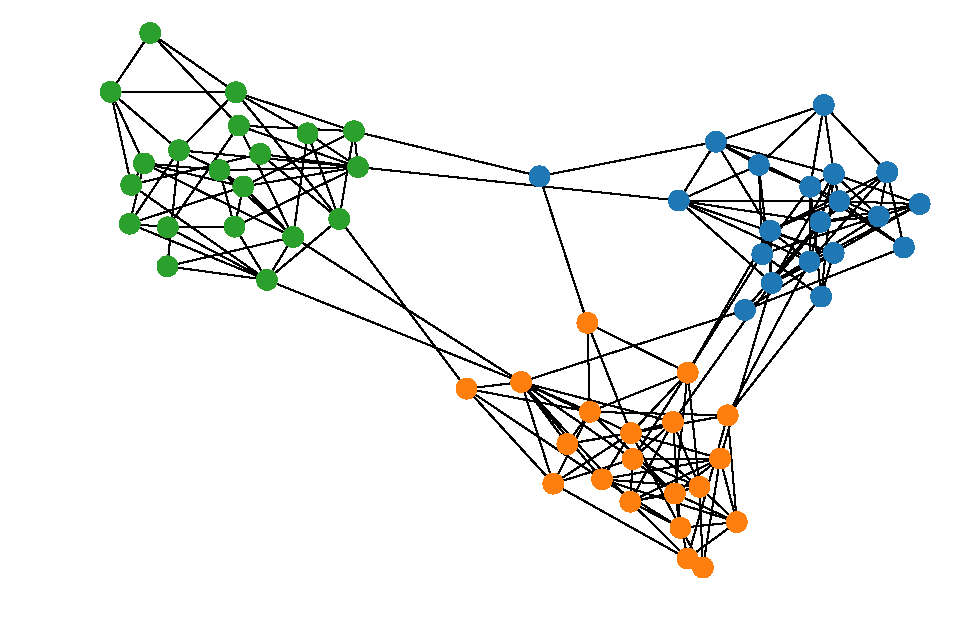
\includegraphics[width=0.7\textwidth]{SBM_example_3clusters.pdf}
   \caption{Example of the stochastic block model with 3 communities}
   \label{fig:sbm_example}
 \end{figure}

The general inference technique, or model fitting procedure, is based on Maximum Likelihood Estimation (MLE). However, even for this simple model there in no exact solution of MLE and computation of this maximum in general case is NP-hard. There exist a number of approximate method based on various optimization algorithms, Monte-Carlo sampling or Bayesian approach \cite{BrianNewman2011}. In the framework of this study we use the MLE estimator given in \cite{Peixoto2014}. 

It is evident that if the connection probabilities are close to each other, the SBM network will resemble the ordinary Erdos-Renyi network. In fact, for the case of SBM with two clusters there exists the detectability threshold given in the following Theorem.
\begin{theorem}\label{thm.detectability_SBM}
The SBM with $n$ nodes and two clusters with symmetric affinity matrix $B$, where $b_{11}=b_{22}=p/n$ and $b_{12}=b_{12}=q/n$, can be inferred with high probability iff $(p-q)^2> 2(p+q)$. When $(p-q)^2 < 2(p+q)$, any algorithm will fail to infer the original SBM with high probability. 
\end{theorem}

In the following subsection we describe the community detection methods used in our study.

\section{Community detection methods}

\subsection{Greedy modularity maximization}
The method is presented in \cite{Clauset2004} and, as suggested by its name, it is designed to find a partition of the network by maximizing the modularity function of the partition. Initially, at the start of the algorithm, it is assumed that all nodes belong to its own communities and two communities are merged if this increases modularity. The algorithm stops when no merge is further possible. The algorithm was proposed as a fast approach for very large networks with complexity $O(md\log n)$, where $m$ is the number of edges, $n$ is the number of nodes and $d$ is the diameter, which for the case of sparse real-life networks turns into $O(n \log^2 n)$.

\subsection{Louvain method}
The method is presented in \cite{Blondel2008} and is one of the most commonly used methods for community detection in large networks and it is also based on maximizing modularity function. The optimization is performed in two steps. First, the method looks for ``small'' communities by optimizing modularity locally. Second, it aggregates nodes belonging to the same community and builds a new network whose nodes are the communities. These steps are repeated iteratively until a maximum of modularity is attained and a hierarchy of communities is produced. Although the exact computational complexity of the method is not known, the method seems to run in time $O(n \log n)$ with most of the computational effort spent on the optimization at the first level.

\subsection{Infomap}
The method is described in \cite{Rosvall2008} and uses random walks and information-theoretic measures to capture the community structure of networks. The method is based on an observation that a random walker is prone to be trapped within the communities. The algorithm is designed to find the efficient way to encode the trajectories of a random walker using Huffman codes. The quality function is given by a so-called ``map equation'', which incorporates Shannon entropy of the code to accommodate the walker inside the community, as well as the inter-community jumps. The method has shown itself very efficient and runs in $O(n)$ time.

\subsection{Node2Vec + K-means}
We apply our method to the problem of community detection in networks. The node2vec algorithm gives the embedding of the graph into the real space $\mathbb{R}^d$, such that the nodes which are close to each other in the graph are mapped to the close points in the embedding space. Hence, the clustering of nodes can be obtained by any vector clustering algorithm and for our study we used the \textit{k-means clustering} \cite{Macqueen1967}. The choice of the optimal number of clusters is then found using \textit{silhouette analysis}. Silhouette analysis can be used to study the separation distance between the resulting clusters. The silhouette plot displays a measure of how close each point in one cluster is to points in the neighboring clusters and thus provides a way to assess parameters like number of clusters visually. This measure has a range of $[-1, 1]$. 
\begin{figure}[ht]
 \centering
    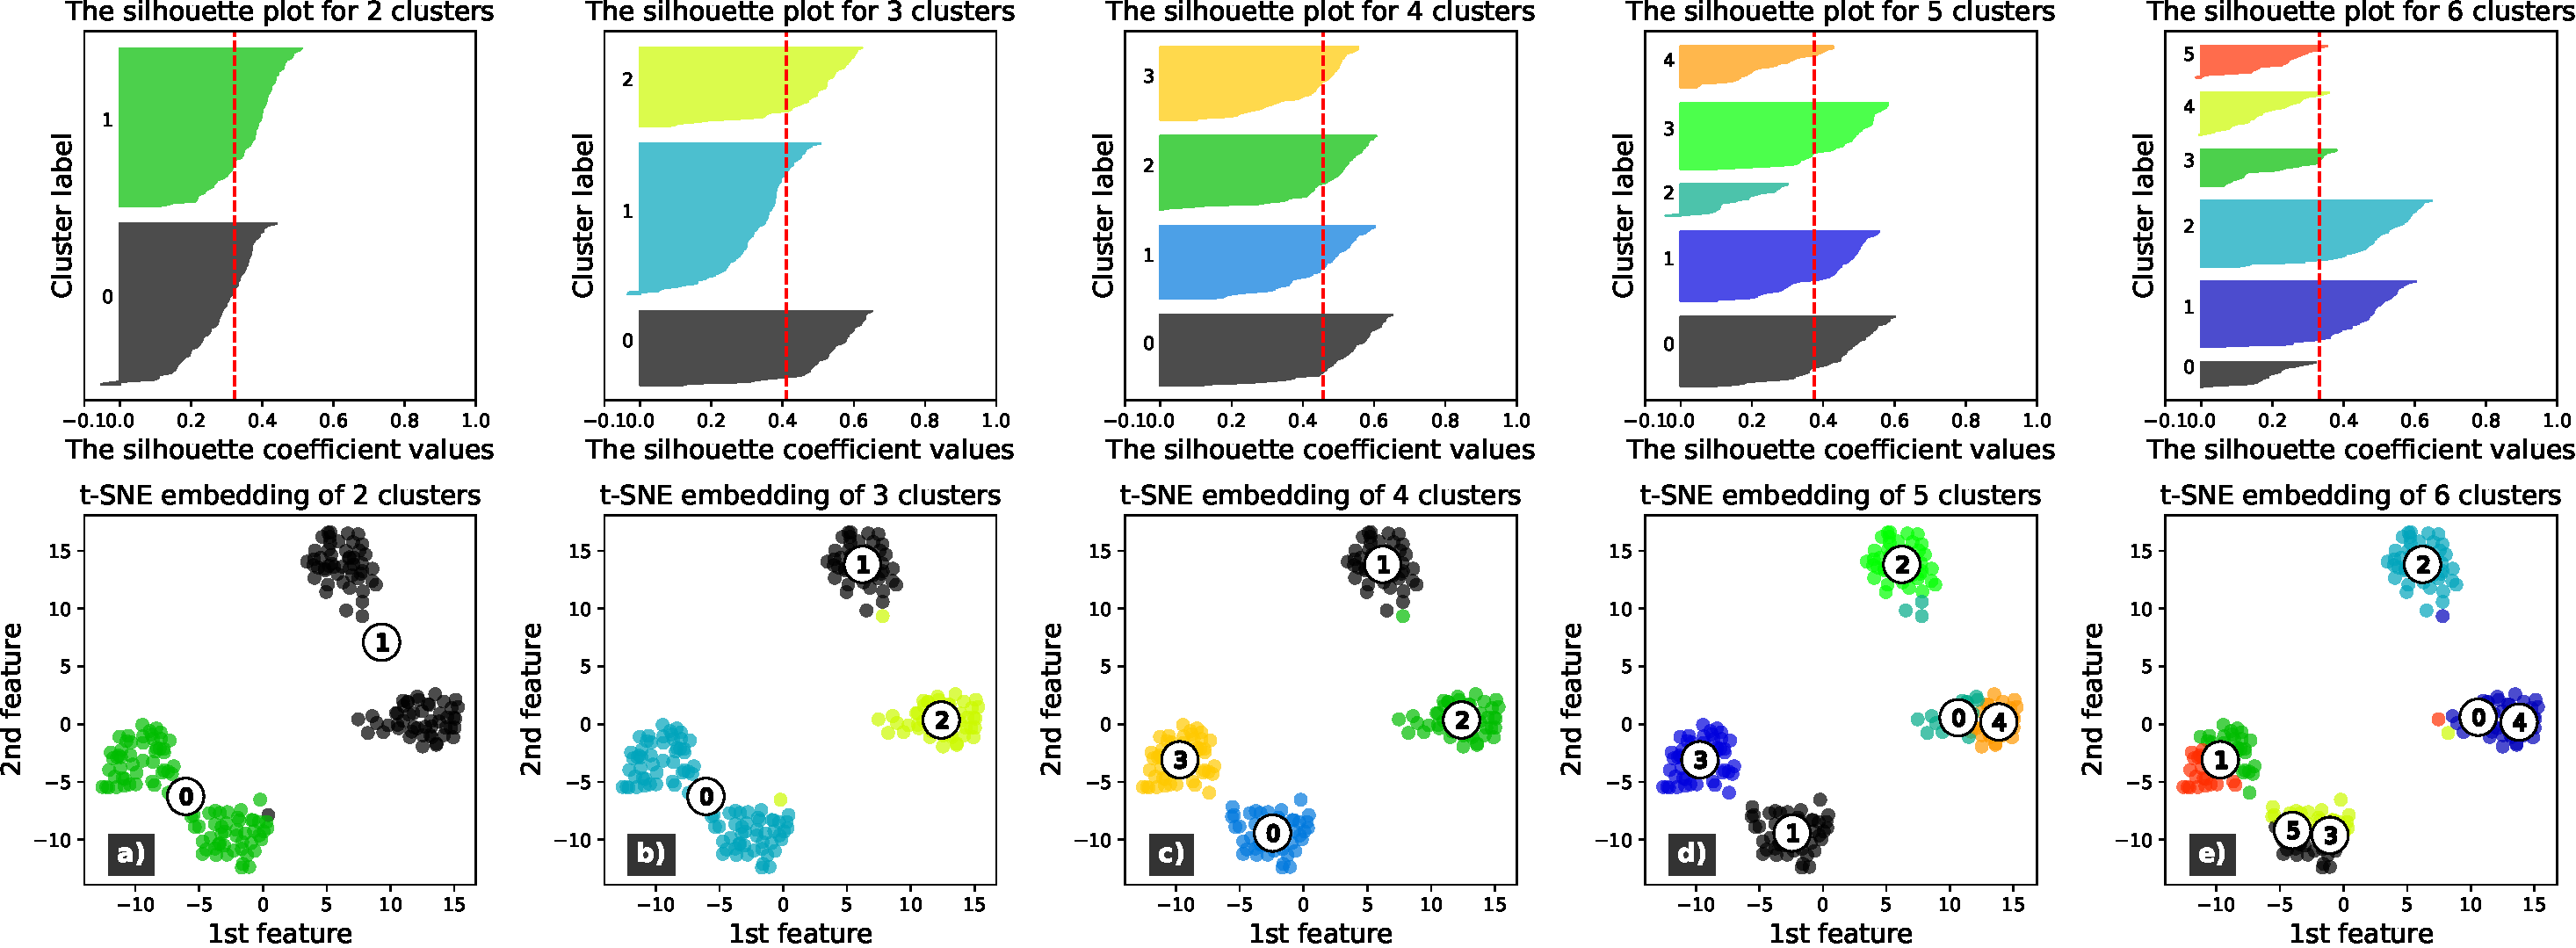
\includegraphics[width=1\textwidth]{avg_silhouette_with_4_clusters_50.pdf}
   \caption{Silhouette plot and t-SNE representation of the embedding for SBM with 4 clusters and results of k-means clustering into a) two to e) six clusters. Red line denotes the average silhouette coefficient, which is maximized in the ground truth of four clusters.}
   \label{fig:silhouette_example}
 \end{figure}

Silhouette coefficients (as these values are referred to as) near $+1$ indicate that the sample is far away from the neighboring clusters. A value of $0$ indicates that the sample is on or very close to the decision boundary between two neighboring clusters and negative values indicate that those samples might have been assigned to the wrong cluster. We use the average silhouette score for a clustering to measure its fitness and choose a partition with the largest average score. 

On Figure \ref{fig:silhouette_example} we show the example of the silhouette coefficient calculation for the case of the SBM with four planted clusters. The upper plots show the silhouette scores for the nodes in the assigned cluster by k-means algorithms, dashed red line denotes the average silhouette coefficient of the partitioning. The lower set of plots show the t-SNE two dimensional embedding of the node2vec embedding of the graph nodes. We may notice that cluster structure is well pronounced. 

\section{Results}
\subsection{Comparison of the clustering algorithms}
In this section we compare the performance of clustering algorithms on the test networks generated from SBM with different number of clusters. For the sake of tractability, we shall use the symmetric SBM with uniform cluster size of 100 nodes and with affinity matrix $B$ given by $b_{ii}=\alpha$, where $1\leq i\leq k$ and $b_{ij} = \beta$, where $1\leq i\neq j\leq k$. We choose accuracy of the partitioning as the performance measure for the analysis. Given two vector $y_{true}$ and $y_{pred}$, accuracy measure $acc(y_{true}, y_{pred})$ is defined as the maximum of the fraction of matching labels (coordinatewise) over all possible relabellings. This measure is widely used in classification tasks using machine learning algorithms. If labels are unique for both vectors, the minimum value of $acc(y_{true}, y_{pred})$ is $1/\text{number of labels}$, which corresponds to purely random labelling. When labels are different, e.g. when a clustering algorithm found more clusters than it is  actually present in the data, then minimum value of $acc(y_{true}, y_{pred})$ may attain lower values. 
\begin{figure}[ht]
 \centering
    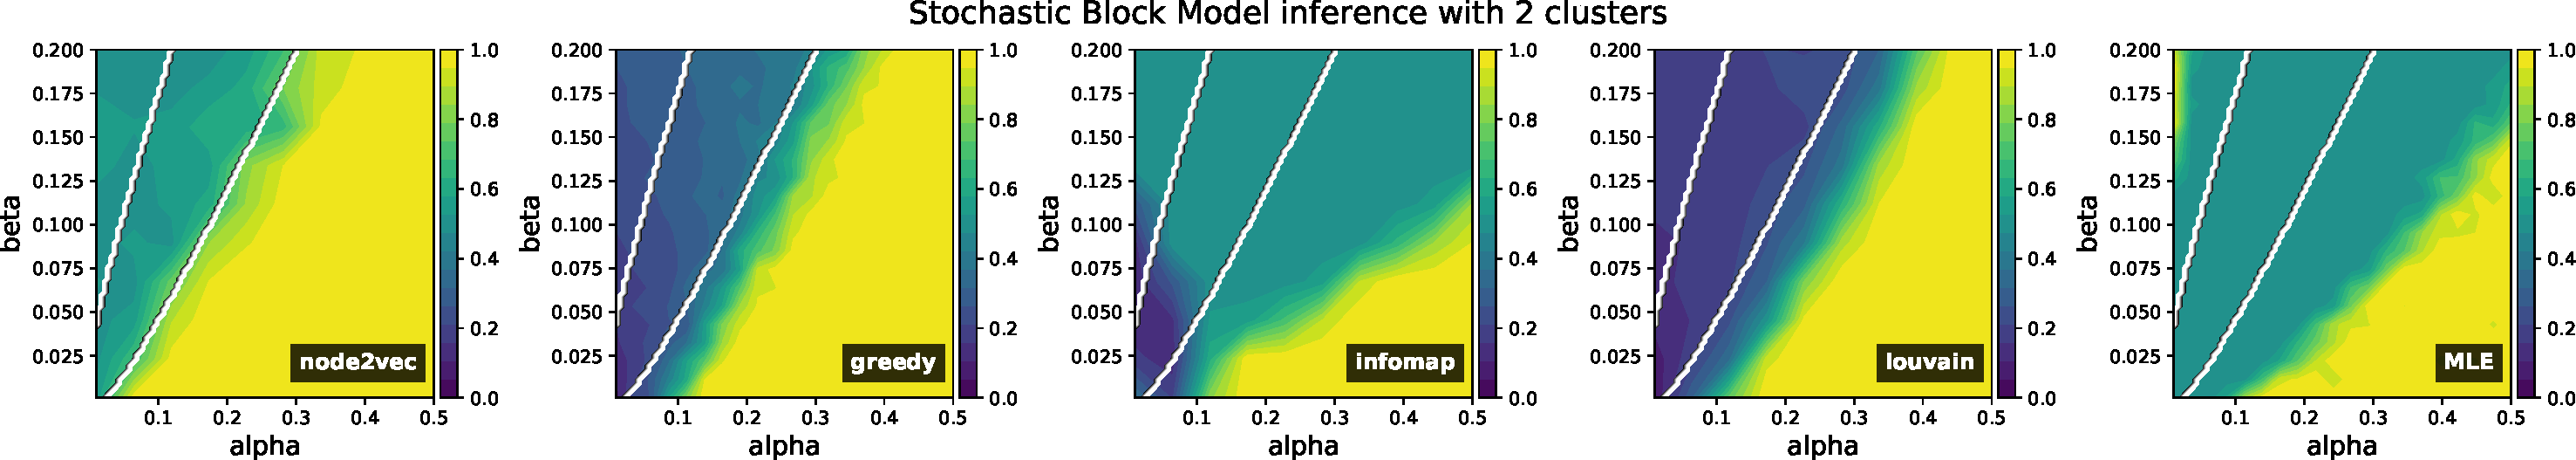
\includegraphics[width=1\textwidth]{clustering_SBM_heatmap_2_clusters.pdf}
   \caption{Comparison of the accuracies of community detection algorithms for symmetric SBM with 2 clusters over a range of parameter values $\alpha$ and $\beta$. White lines represent theoretical detectability thresholds from Theorem \ref{thm.detectability_SBM}.}
   \label{fig:comparison_clustering_2clusters}
 \end{figure}
 
On Figure \ref{fig:comparison_clustering_2clusters} we show the results of the partitioning accuracy of the symmetric SBM with two clusters of 100 nodes over a range of parameters $\alpha$ and $\beta$. According to the Theorem \ref{thm.detectability_SBM} we also plot the region of the theoretical detectability of clusters with white lines. It is notable that our method outperforms the benchmark methods within the whole range of $(\alpha,\,\beta)$, except the upper left corner, where the Maximum Likelihood Estimation finds the ``inverse'' clusters, which correspond to high values of $\beta$ and small $\alpha$. In the undetectable region the node2vec + k-means and MLE place all the nodes into one cluster, however Louvain and greedy optimisation detect more communities that result in lower accuracy values.

We perform the same experiment for symmetric SBM with four and six clusters and the results are shown on Figures \ref{fig:comparison_clustering_4clusters} and \ref{fig:comparison_clustering_6clusters}. The performance of node2vec + k-means clustering seem to be consistent over the increase in the number of clusters. It is worth to note that Louvain algorithm shows similar detectability power, however it cannot detect clusters in the anti-planted partition region in the upper left corner.
 
 \begin{figure}[ht]
 \centering
    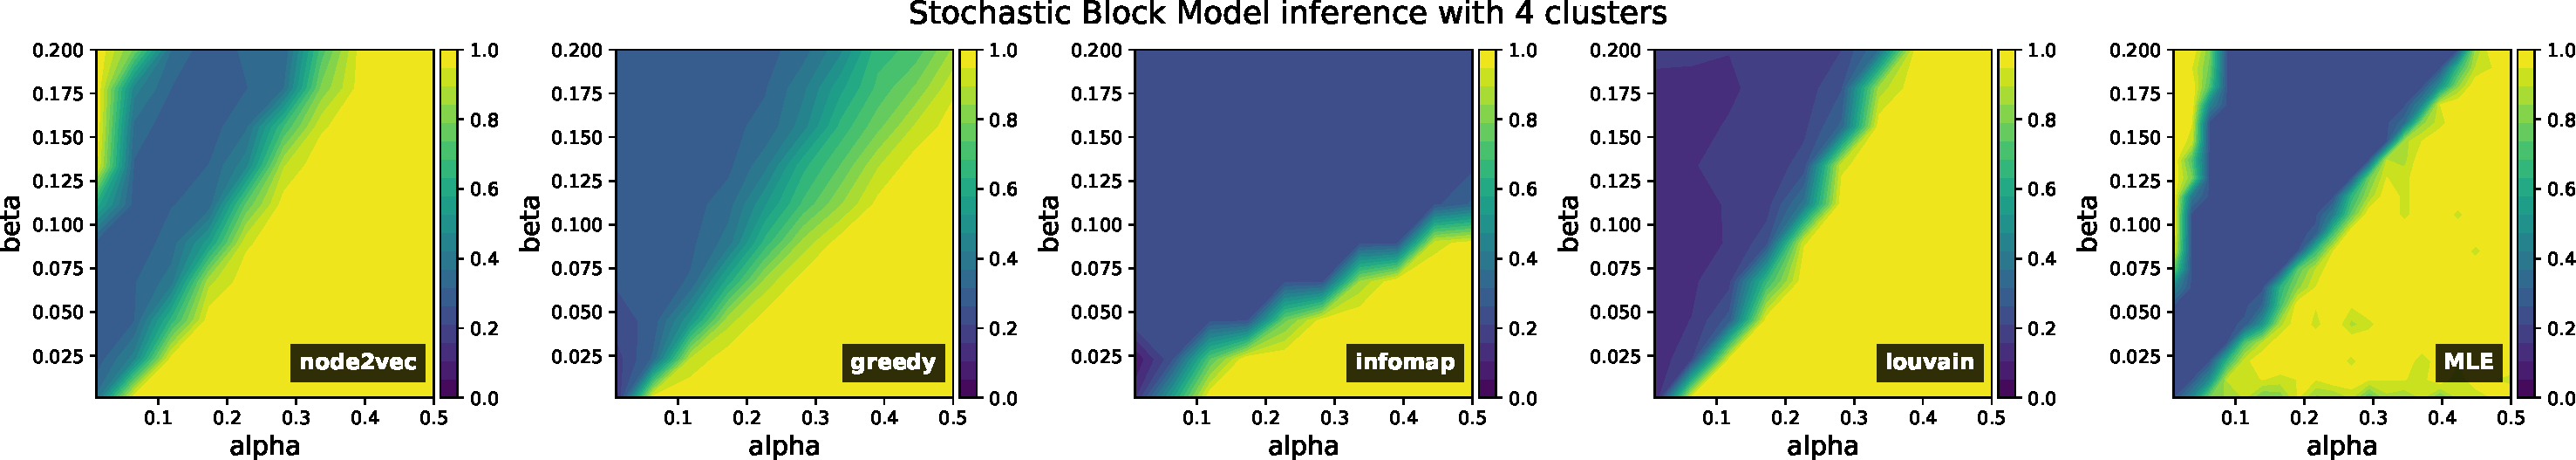
\includegraphics[width=1\textwidth]{clustering_SBM_heatmap_4_clusters.pdf}
   \caption{Comparison of the accuracies of community detection algorithms for symmetric SBM with 4 clusters over a range of parameter values $\alpha$ and $\beta$.}
   \label{fig:comparison_clustering_4clusters}
 \end{figure}
 
  \begin{figure}[ht]
 \centering
    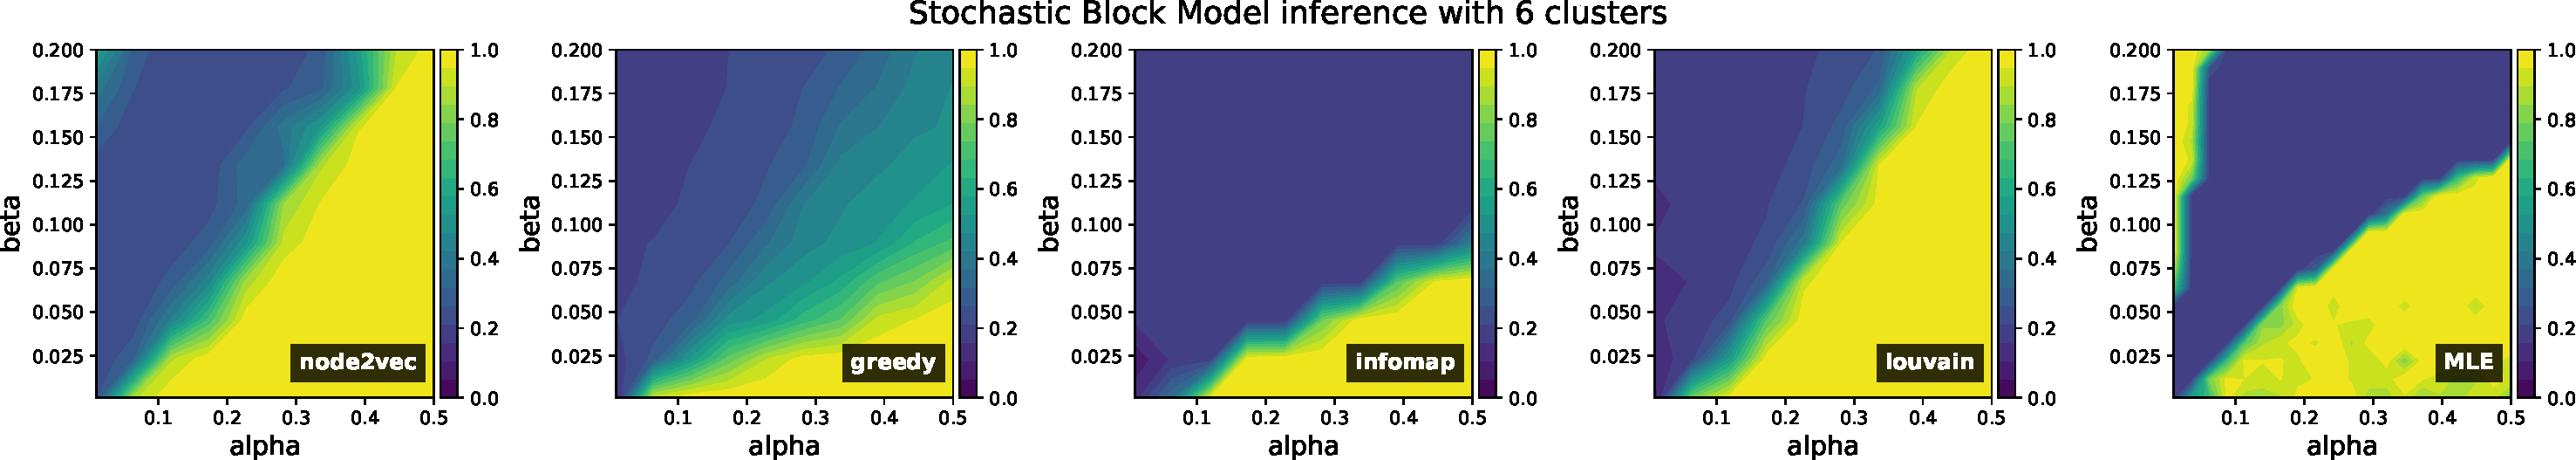
\includegraphics[width=1\textwidth]{clustering_SBM_heatmap_6_clusters.pdf}
   \caption{Comparison of the accuracies of community detection algorithms for symmetric SBM with 6 clusters over a range of parameter values $\alpha$ and $\beta$.}
   \label{fig:comparison_clustering_6clusters}
 \end{figure}
 
\subsection{Parameters of node2vec embedding and clustering accuracy}
The algorithm node2vec has three essential input parameters that define the embedding: 1) number of dimensions in the target space, 2) length of a random walk, 3) number of generated walks. It is intuitive that higher parameter values may result in better embedding, but may carry additional computational load. Thus, we glance on the influence of these parameters on the accuracy of the algorithm. On Figure \ref{fig.params_node2vec} we represent the accuracy of clustering of the symmetric SBM with two clusters of 100 nodes each and $\alpha=0.2$ and $\beta = 0.08$ (near the detectability threshold). The results are somewhat expected - the larger the embedding dimensionality, the more structural information is encoded, the larger the walk length - the larger part of the graph can be explored, thus resulting in better description of the mesoscale structure and number of walks ensure diversity of the captured information.
\begin{figure}[ht]
\centering
\begin{minipage}[b]{0.32\textwidth}
\centering
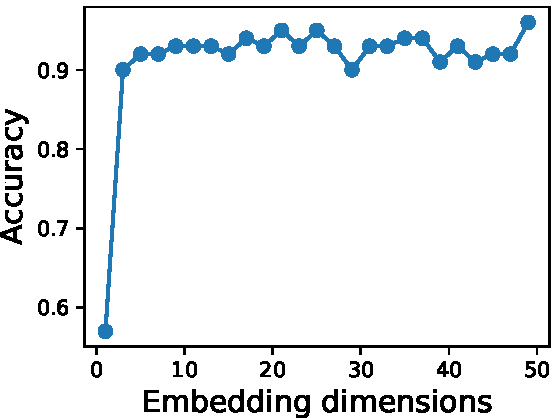
\includegraphics[width = 0.8\linewidth]{node2vec_dimensions_accuracy_100.pdf}
%\caption*{Node2Vec embedding: number of dimensions vs. accuracy}
\end{minipage}\hfill
\begin{minipage}[b]{0.32\textwidth}
\centering
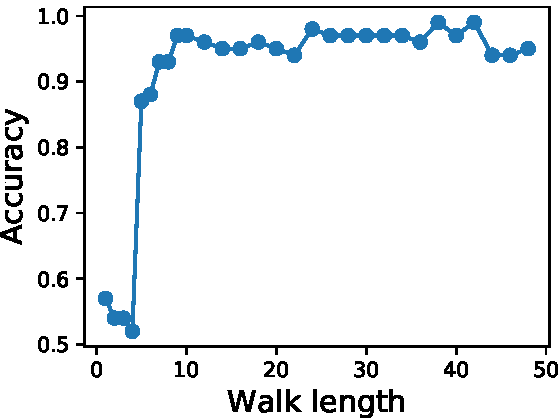
\includegraphics[width =0.8\linewidth]{node2vec_walk_length_accuracy_100.pdf}
%\caption*{Node2Vec embedding: walk length vs. accuracy}
\end{minipage}\hfill
\begin{minipage}[b]{0.32\textwidth}
\centering
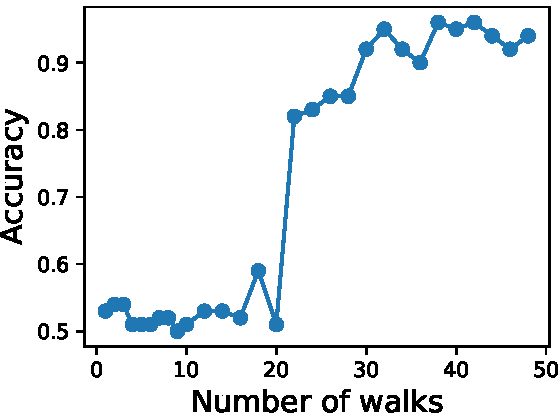
\includegraphics[width =0.8 \linewidth]{node2vec_num_walks_accuracy_nodes_100.pdf}
%\caption*{Node2Vec embedding: number of walks vs. accuracy}
\end{minipage}
\caption{Node2Vec embedding: number of dimensions, walk length and number of walks vs. accuracy}
\label{fig.params_node2vec}
\end{figure}

\subsection{Transformation of the distance matrix}
It is commonly expected that embedding of the graphical metric space to the real space will loose structural information of the original graph. We question this common hypothesis by providing the analysis of distance matrices of the graph before and after embedding. The distance matrix is the $n\times n$ matrix with $(i,j)$ entry is basically the distance between node $i$ and $j$. For the original graph we use the shortest path metric, for the embedding we use $\mathcal{L}^2$ Euclidean norm. 

We sample the SBM with four clusters of 500 nodes and symmetric connection probabilities $\alpha=0.2$ and $\beta = 0.05$. It turns out that the distance between nodes saturates after embedding (see Figure \ref{fig:distance_matrices}) - the nodes which were closer in the original graph become closer in the embedding space and those that were far turn even farther away. This may be explained by the fact that the closer nodes inside the cluster have more chance to appear in the trajectory of a random walker, in comparison to the nodes in other communities. Since node2vec evaluates the embedding position based on the frequency of a node in random walks, we obtain such saturation effect.

 \begin{figure}[ht]
 \centering
    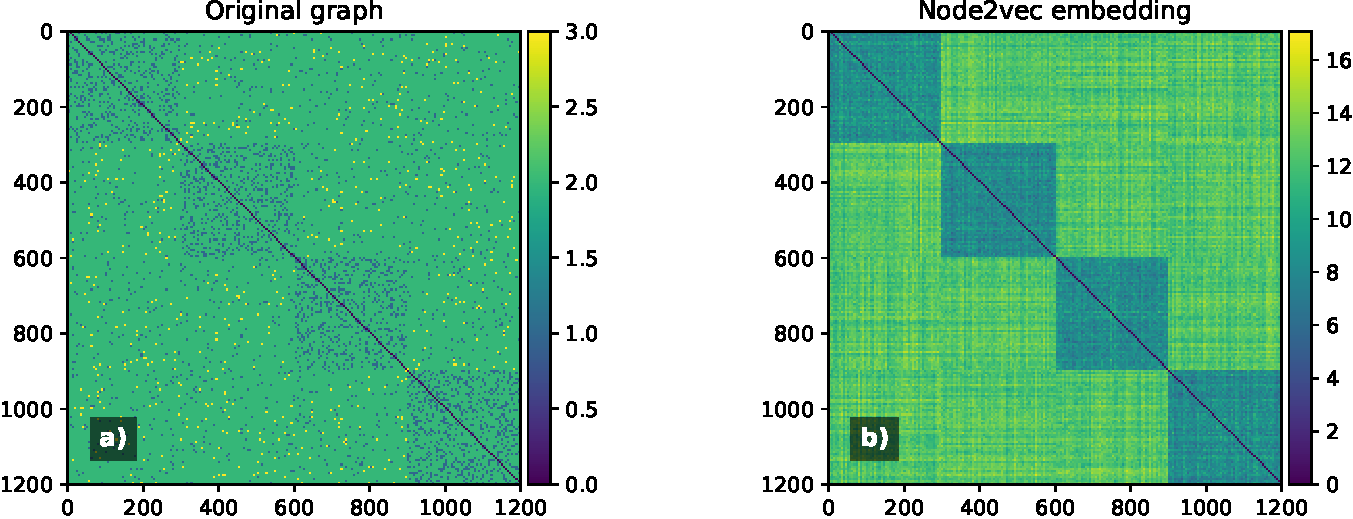
\includegraphics[width=0.8\textwidth]{distance_matrix_4_clusters.pdf}
    \caption{a) The original distance matrix of the SBM network with four clusters; b) the distance matrix of the node2vec embedding. Community structure saturates after the embedding.}
   \label{fig:distance_matrices}
 \end{figure}


